\documentclass[french]{book}

\usepackage[top=2cm, bottom=2cm, left=2cm, right=2cm]{geometry}

\usepackage[T1]{fontenc}
\usepackage[utf8]{inputenc}
\usepackage{babel}
\usepackage{pdflscape}
\usepackage{titlesec}
\usepackage{multicol}
\usepackage[inline]{enumitem}
\usepackage{amsmath, amsthm, amssymb}
\usepackage[squaren, Gray]{SIunits}
\usepackage{mathrsfs}
\usepackage{float}
\usepackage{array}
\usepackage{caption}
\usepackage{hyperref} % Liens dans la table des matières


% TikZ

\usepackage{tikz}
\usetikzlibrary{babel}
\usetikzlibrary{calc}
\usetikzlibrary{arrows}
\usetikzlibrary{patterns}
\usetikzlibrary{decorations.pathmorphing, decorations.markings}
\usetikzlibrary{positioning}
\usetikzlibrary{optics}


% "north east hatch" pattern
\makeatletter
\tikzset{% customization of pattern 
        hatch distance/.store in=\hatchdistance,
        hatch distance=5pt,
        hatch thickness/.store in=\hatchthickness,
        hatch thickness=5pt
        }
\pgfdeclarepatternformonly[\hatchdistance,\hatchthickness]{north east hatch}% name
    {\pgfqpoint{-1pt}{-1pt}}% below left
    {\pgfqpoint{\hatchdistance}{\hatchdistance}}% above right
    {\pgfpoint{\hatchdistance-1pt}{\hatchdistance-1pt}}%
    {
        \pgfsetcolor{\tikz@pattern@color}
        \pgfsetlinewidth{\hatchthickness}
        \pgfpathmoveto{\pgfqpoint{0pt}{0pt}}
        \pgfpathlineto{\pgfqpoint{\hatchdistance}{\hatchdistance}}
        \pgfusepath{stroke}
    }
\makeatother

\tikzset{>=stealth}
\tikzset{schema/.style={rounded corners=#1, fill=lightgray, draw, inner sep=0pt},
         schema/.default=4pt}
\tikzset{bati/.style={pattern=north east hatch, hatch distance=7pt, hatch thickness=1.2pt, preaction={fill=lightgray}}}
\tikzset{ressort/.style 2 args={decorate, decoration={coil,aspect=#1,segment length=#2,amplitude=3mm}}}


% Pour les spectres d'émission / d'absorption

\usepackage{pgf-spectra}


% Couverture

\ifpdf
	\usepackage{pdfcolmk}
\fi

\ifxetex
	\usepackage{fontspec}
\fi

\usepackage{url}
\usepackage{graphicx}
\usepackage{pifont}

\newlength{\drop}

\newcommand*{\mytitle}{\begin{titlepage}
\begingroup
\drop = 0.13\textheight
\centering
\vspace*{\drop}
{\Huge Physique (\textsc{mpsi})}\\[\baselineskip]
{\Huge\itshape Année scolaire 2017-2018}\\[3\baselineskip]
{\Large \textit{Cours de} \textsc{N. Tancrez}}\par
\vfill
{\begin{center}\includegraphics[scale=1.5]{SL.png}\end{center}}
\vspace*{1cm}
{\Large Lycée Saint-Louis}\par
\vspace*{\drop}
\endgroup
\end{titlepage}}



% Style des sections

\titleformat{\chapter}
[frame] % format
{\vspace*{5cm}\Huge} % format du texte
{\thechapter} % format du label
{1cm} % séparation
{\centering\sffamily} % avant
[\thispagestyle{empty}] % après


% pour la table des matières
\titleformat{name=\chapter, numberless}
[display] % format
{\Large\bfseries} % format du texte
{\titlerule} % format du label
{-7ex} % séparation
{\centering\MakeUppercase} % avant


\titleformat{\section}
[block] % format
{\LARGE\bfseries} % format du texte
{\thesection} % format du label
{8pt} % séparation
{\centering} % avant

\titleformat*{\subsection}{\Large\bfseries}


\renewcommand{\thechapter}{\Roman{chapter}}
\renewcommand{\thesection}{\arabic{section}.}
\renewcommand{\thesubsection}{\Roman{subsection}}

\pagestyle{plain} % Numéro de page en bas de la page
\setcounter{tocdepth}{1} % On ne veut que les sections

% Math environments

\newtheorem*{lemme}{Lemme}
\newtheorem*{theoreme}{Théorème}
\newtheorem*{propriete}{Propriété}
\newtheorem*{proprietes}{Propriétés}

\theoremstyle{definition}
\newtheorem*{definition}{Définition}
\newtheorem*{definitions}{Définitions}
\newtheorem*{exemple}{Exemple}
\newtheorem*{exemples}{Exemples}
\newtheorem*{experience}{Expérience}
\newtheorem*{vocabulaire}{Vocabulaire}

\theoremstyle{remark}
\newtheorem*{remarque}{Remarque}


% Math macros

\usepackage{mathtools}

\DeclarePairedDelimiter\abs{\lvert}{\rvert}
 
\makeatletter
\let\oldabs\abs
\def\abs{\@ifstar{\oldabs}{\oldabs*}}
\makeatother


\newcommand*\dif{\mathop{}\!\mathrm{d}}


% Conventions du cours

\newcommand*{\point}[1]{\mathrm{#1}}
\newcommand*{\droite}[1]{\mathrm{#1}}
\newcommand*{\systeme}[1]{\mathrm{#1}}
\newcommand*{\vecteur}[1]{\overrightarrow{#1}}
\newcommand*{\algebrique}[1]{\overline{#1}}


\newcommand*{\tdef}[1]{\textbf{#1}}
\newcommand*{\imp}[1]{\emph{#1}}
\newcommand*{\abr}[1]{\textsc{#1}}



% Où chercher les fichiers

\makeatletter
\def\input@path{{01_signaux_harmoniques_propagation/}, {02_optique_geometrique/}}
\makeatother

\newcommand{\cours}[2]
{\begin{landscape}
\begin{multicols*}{2}[\section{#1}]
\input{#2}
\end{multicols*}
\end{landscape}}


%%%%%%% Document %%%%%%%

\begin{document}

% Titre

\mytitle

\tableofcontents

\chapter{\textsc{Signaux harmoniques et propagation}}

\cours{Oscillateur harmonique}{01_oscillateur_harmonique}
\cours{Propagation d'un signal}{02_propagation_signal}
\cours{Ondes progressives sinusoïdales}{03_ondes_progressives_sinusoidales}
\cours{Interférences}{04_interferences}
\cours{Ondes stationnaires}{05_ondes_stationnaires}
\cours{Diffraction}{06_diffraction}

% TODO : ordres de grandeur

\chapter{\textsc{Optique géométrique}}

\cours{Description ondulatoire de la lumière}{01_description_ondulatoire_lumiere}
\cours{Modèle géométrique de la lumière}{02_modele_geometrique_lumiere}
\cours{Systèmes optiques}{03_systemes_optiques}
\cours{Systèmes centrés}{04_systemes_centres}
\cours{Foyers et plans focaux}{05_foyers_plans_focaux}
\cours{Miroir et dioptre plan}{06_miroir_dioptre}



\begin{landscape}
\begin{multicols*}{2}[\section{Lentilles minces sphériques}]

\subsection{Présentation générale}

\begin{definition}
On appelle \tdef{lentille sphérique} la portion de l'espace délimitée par l'intersection de deux milieux situés de part et d'autre de :

\begin{itemize}
\item deux dioptres sphériques; l'axe optique de la lentille passe alors par les deux centres $\point{C}_1$ et $\point{C}_2$ des dioptres sphériques;
\item un dioptre plan et un dioptre sphérique.
\end{itemize}

\begin{figure}[H]
\begin{center}
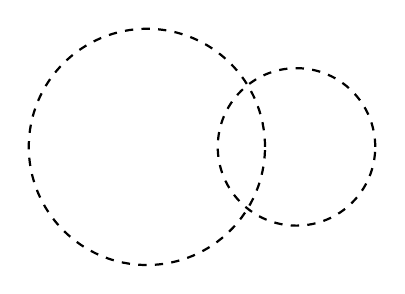
\begin{tikzpicture}[thick]
\coordinate (C1) at (-1.2,0);
\coordinate (C2) at (0.7,0);

\draw [dashed] (C1) circle [radius=1.5];
\draw [dashed] (C2) circle [radius=1];

\end{tikzpicture}
\end{center}
\end{figure}
\end{definition}

\begin{propriete}
Une \imp{lentille sphérique} est dite \tdef{mince} (ou \tdef{\abr{lms}}) lorsque son épaisseur $e$ est très petite à la fois devant les rayons de courbure $R_1$ et $R_2$ des dioptres qui la délimitent, et devant leur différence :

\begin{center}
\begin{itemize*}[itemjoin=\qquad]
\item $ e \ll R_1$
\item $ e \ll R_2$
\item $ e \ll \abs{R_1 - R_2}$
\end{itemize*}
\end{center}

\noindent Dans ce cas, $\point{O} \simeq \point{S}_1 \simeq \point{S}_2$ est appelé \tdef{centre de la lentille}.

\end{propriete}

\subsection{Stigmatisme et aplanétisme}

\begin{propriete}

Dans les \imp{\abr{lms}}, il y a absence de stigmatisme (et donc d'aplanétisme) rigoureux. Toutefois, il y a stigmatisme et aplanétisme approché dans les \imp{conditions de Gauss}.

\end{propriete}

\end{multicols*}
\end{landscape}



\begin{landscape}
\begin{multicols*}{2}[\section{Propriétés des \abr{lms} dans les conditions de Gauss}]

\begin{propriete}
Un rayon passant par le \imp{centre optique} d'une \abr{lms} n'est pas dévié.
\end{propriete}

\begin{definitions}
On définit la \tdef{distance focale objet} $f$ (resp. \tdef{distance focale image} $f'$) d'une \abr{lms} par :
\[f = \algebrique{\point{O}\point{F}} \quad \text{(resp. } f' = \algebrique{\point{O}\point{F'}} \text{)}\]
\end{definitions}

\begin{propriete}
Les distances focales image et objet d'une \imp{\abr{lms}} sont opposées :
\[f' = -f\]
\end{propriete}

\begin{definition}
La \tdef{vergence} $V$ d'une \abr{lms} est définie par : 
\[V = \frac{1}{f'}\]
\end{definition}

\begin{remarque}
$V$ s'exprime généralement en \tdef{dioptries} $\delta \equiv \reciprocal\meter$.
\end{remarque}

\begin{propriete}
Une \imp{\abr{lms} convergente} (resp. \imp{divergente}) est caractérisée par :
\[f' > 0 \quad \text{(resp. } f' < 0 \text{)} \qquad \text{ou} \qquad V > 0 \quad \text{(resp. } V < 0 \text{)}\]
\noindent Ainsi ses foyers objet et image sont réels (resp. virtuels).
\end{propriete}

\begin{proprietes}
Le conjugué d'un point objet $\point{\phi}$ situé dans le plan focal objet (resp. d'un point image $\point{\phi'}$ situé dans le plan focal image) est un point image à l'infini hors axe optique dans la direction de $\droite{\left(\point{\phi}\point{O}\right)}$ (resp. $\droite{\left(\point{\phi'}\point{O}\right)}$) :
\[\point{\phi} \stackrel{\mathscr{L}}{\longmapsto} \point{A'}_{\infty}  \qquad \text{(resp. } \point{A}_{\infty} \stackrel{\mathscr{L}}{\longmapsto} \point{\phi'} \text{)}\]
\end{proprietes}

\begin{theoreme}
On a les \tdef{formules de Newton}
\end{theoreme}

\begin{theoreme}[Relations de Newton]

\[
\frac{\algebrique{\point{A'}\point{B'}}}{\algebrique{\point{A}\point{B}}} = \gamma 
= \frac{\algebrique{\point{F}\point{O}}}{\algebrique{\point{F}\point{A}}}
= \frac{f'}{\algebrique{\point{F}\point{A}}}
= \frac{\algebrique{\point{F'}\point{A'}}}{\algebrique{\point{F'}\point{O}}}
= \frac{\algebrique{\point{F'}\point{A'}}}{-f'}
\quad \text{grandissement}
\]

\[
\algebrique{\point{F'}\point{A'}} \cdot \algebrique{\point{F}\point{A}}
= \algebrique{\point{F'}\point{O}} \cdot \algebrique{\point{F}\point{O}} 
= -{f'}^2
\quad \text{relation de conjugaison}
\]

\end{theoreme}

\begin{theoreme}[Relations de Descartes]

\[
\frac{\algebrique{\point{A'}\point{B'}}}{\algebrique{\point{A}\point{B}}} = \gamma 
= \frac{\algebrique{\point{O}\point{A'}}}{\algebrique{\point{O}\point{A}}}
\quad \text{grandissement}
\]

\[
\frac{1}{\algebrique{\point{O}\point{A'}}} - \frac{1}{\algebrique{\point{O}\point{A}}}
= \frac{1}{\algebrique{\point{O}\point{F'}}}
= \frac{1}{f'}
\quad \text{relation de conjugaison}
\]

\end{theoreme}

\begin{propriete}

Pour former l'image réelle sur un écran d'un objet réel par une lentille convergente de distance focale image $f'$, il est nécessaire que la distance $D$ entre l'objet et l'écran vérifie : \imp{$D \geq 4f'$}

\end{propriete}

\begin{theoreme}[Lentilles accolées]
Deux \imp{\abr{lms}} $\mathscr{L}_1$ et $\mathscr{L}_2$ \imp{accolées} de vergences $V_1$ et $V_2$ se comportent comme une \abr{lms} $\mathscr{L}$ de vergence $V$ telle que :
\[V = V_1 + V_2\]
\end{theoreme}

\begin{definition}

Le \tdef{grossissement} optique correspond au  rapport entre l’angle $\alpha'$ sous lequel est vue l’image formée par le système optique et l’angle $\alpha$ sous lequel est vu l’objet (par rapport à l'axe optique). \imp{$G = \frac{\alpha'}{\alpha}$}

\end{definition}

\end{multicols*}
\end{landscape}



\chapter{\textsc{Thermodynamique}}

\end{document}
